%REPORT TEMPLATE
%AUTHOR: RUI QU  
%EMAIL: RQU@KTH.SE 

%----------------------------------------------------------------------------------------
%	PACKAGES AND DOCUMENT CONFIGURATIONS
%----------------------------------------------------------------------------------------

\documentclass{article}

%---Basic---
\usepackage{natbib} % Required to change bibliography style to APA
\usepackage{amsmath} % Required for some math elements 
\setlength\parindent{0pt} % Removes all indentation from paragraphs
\usepackage{listings}%Insert code
\usepackage{times} % Uncomment to use the Times New Roman font
\newcommand*{\dif}{\mathop{\mathrm{d}}\!} %differential


%---Table---
\usepackage{multirow}%Table
\usepackage{booktabs}%Table Triple-lines
\usepackage{siunitx} % Provides the \SI{}{} and \si{} command for typesetting SI units

%---Figure---
\usepackage{graphicx} % Required for the inclusion of images
\usepackage{subfigure} % Required for multiple images
\usepackage{float} 

%---Pseudo-code in LaTeX---
\usepackage{algorithm}
\usepackage{algpseudocode}
\usepackage{amsmath}
\renewcommand{\algorithmicrequire}{\textbf{Input:}}  % Use Input in the format of Algorithm
\renewcommand{\algorithmicensure}{\textbf{Output:}} % Use Output in the format of Algorithm

%---Appendix---
\usepackage{appendix}
\newcommand{\upcite}[1]{\textsuperscript{\textsuperscript{\cite{#1}}}} %Upcite

%----------------------------------------------------------------------------------------
%	DOCUMENT INFORMATION
%----------------------------------------------------------------------------------------

\begin{document}

\title{CS-E4950 Computer Vision\\Exercise Round 5}                  
\author{Rui Qu\\rui.qu@aalto.fi}
\maketitle

% If you wish to include an abstract, uncomment the lines below
% \begin{abstract}
% Abstract text
% \end{abstract}

%----------------------------------------------------------------------------------------
%	SECTION 1
%----------------------------------------------------------------------------------------

\section*{Exercise 1 Solution}

\subsection*{1.1}
\begin{figure}[H]
\centering  
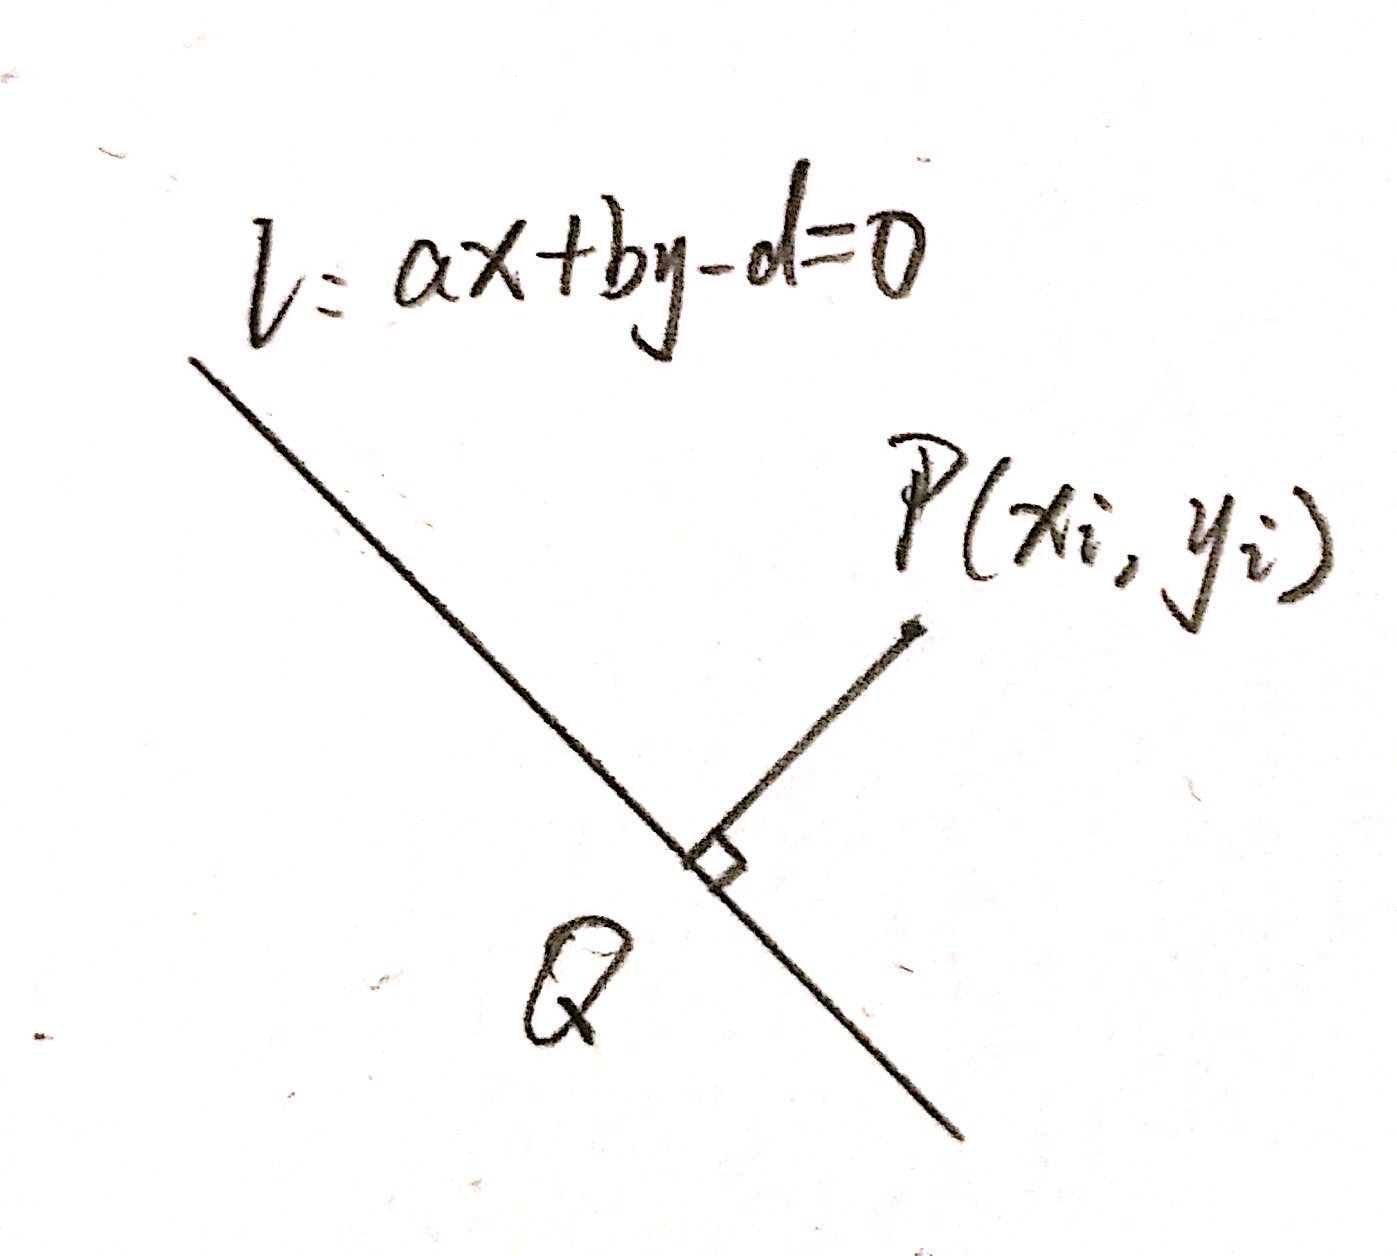
\includegraphics[scale=0.08]{1.png}
%\caption{title}
\label{fig: label}
\end{figure}
Given a line $l:\ ax+by-d=0$ and a point $P(x_i,y_i)$, line $PQ$ is perpendicular to line $l$, hence:
\begin{equation}
k_{PQ}\cdot k_l=-1,\ k_{PQ}=\frac{b}{a}
\end{equation}
The equation of line $PQ$ is:
\begin{equation}
y-y_i=\frac{b}{a}(x-x_i)
\end{equation}
The intersection of line $l$ and $PQ$ is:
\begin{equation}
Q(\frac{b^2x_i-aby_o+ad}{a^2+b^2},\ \frac{a^2y_i-abx_i+bd}{a^2+b^2})
\end{equation}
Hence, the distance between point $P$ and line $l$ is:
\begin{equation}
\begin{aligned}
|PQ|&=\sqrt{(\frac{b^2x_i-aby_i+ad}{a^2+b^2}-x_i)^2+(\frac{a^2y_i-abx_i+bd}{a^2+b^2}-y_i)^2}\\
&=\frac{|ax_i+by_i-d|}{\sqrt{a^2+b^2}}
\end{aligned}
\end{equation}
Since $a^2+b^2=1$, the distance is $|ax_i+by_i-d|$.
 
\subsection*{1.2}
Compute the partial derivative:
\begin{equation}
\frac{\partial E}{\partial d}=\sum^n_{i=1}-2(ax_i+by_i-d)
\end{equation}
Set it to zero and solve $d$ in terms of $a$ and $b$:
\begin{equation}
\begin{aligned}
&a\sum^n_{i=1}x_i+b\sum^n_{i=1}y_i-d\sum^n_{i=1}=0\\
&nd=a\sum^n_{i=1}x_i+b\sum^n_{i=1}y_i\\
&d=\frac{a}{n}\sum^n_{i=1}x_i+\frac{b}{n}\sum^n_{i=1}y_i=a\overline{x}+b\overline{y}
\end{aligned}
\end{equation}

\subsection*{1.3}
Substitute $d$ to the formula of $E$:
\begin{equation}
\begin{aligned}
E&=\sum^n_{i=1}(ax_i+by_i-a\overline{x}-b\overline{y})^2\\
&=\left|\left|\begin{bmatrix}x_1-\overline{x}&y_1-\overline{y}\\ \vdots&\vdots\\ x_n-\overline{x}&y_n-\overline{y}\end{bmatrix}
\begin{bmatrix}a\\b\end{bmatrix}\right|\right|^2\\
&=(UN)^T(UN)\\
&=N^TU^TUN
\end{aligned}
\end{equation}

\subsection*{1.4}
Continue the derivation in 1.3:
\begin{equation}
\begin{aligned}
E&=N^TU^TUN\\
&=\begin{bmatrix}a&b\end{bmatrix}\begin{bmatrix}\sum^n_{i=1}(x_i-\overline{x})^2&\sum^n_{i=1}(x_i-\overline{x})(y_i-\overline{y})\\ \sum^n_{i=1}(x_i-\overline{x})(y_i-\overline{y})&\sum^n_{i=1}(y_i-\overline{y})^2\end{bmatrix}\begin{bmatrix}a\\b\end{bmatrix}
\end{aligned}
\end{equation}

Solution to $2(U^TU)N=0$, subject to $||N||^2=1$, eigenvector of $U^TU$
\begin{equation}
\begin{aligned}
&\frac{\dif E}{\dif N}=2(U^TU)N=0\\
&(U^TU)N=0
\end{aligned}
\end{equation}

\end{document}